\documentclass{beamer}
\usepackage{pgf,tikz}
%Module 1:
%Graphs and level sets, vector fields, the tangent space, surfaces, vector fields on surfaces, orientation.
%(Chapters 1 to 5 of \cite{thorpe}) (20 hours)
%Module 2:
%The Gauss map, geodesics, Parallel transport,
%(Chapters 6, 7 & 8 of \cite{thorpe}) (20 hours)
%Module 3:
%The Weingarten map, curvature of plane curves, Arc length and line integrals
%(Chapters 9, 10 & 11 of \cite{thorpe}) (25 hours)
%Module 4:
%Curvature of surfaces and Parametrized surfaces
%(Chapters 12 & 14 of \cite{thorpe}) (25 hours)

%Module 1 - \cite{thorpe} 1, 2, 3, 4, 5
%Module 2 - \cite{thorpe} 6, 7, 8
%Module 3 - \cite{thorpe} 9, 10, 11
%Module 4 - \cite{thorpe} 12, 14
%Missing - 13, 15, 16?

\title{Differential Geometry}
\author{Module I}
\institute{Chapter 2 : Vector Fields}
\begin{document}

\begin{frame}
	\maketitle
\end{frame}

%\chapter{Vector Fields}
\section{Vector Fields}

\begin{frame}{Vector at a point}
\begin{definition}
	A vector $\mathbf{v}$ at a point $p \in \mathbb{R}^{n+1}$ is a pair $\mathbf{v} = (p,v)$ where $v \in \mathbb{R}^{n+1}$.
\end{definition}

\begin{block}{Operations}
\begin{description}
	\item[vector addition] $\mathbf{v} + \mathbf{w} = (p,v) + (p,w) = (p,v+w)$.
	\item[scalar multiplication] Let $c \in \mathbb{R}$, then $c \mathbf{v} =  c(p,v) = (p,cv)$.
	\item[dot product] $\mathbf{v}\cdot \mathbf{w} = (p,v)\cdot(p,w) = v \cdot w$
	\item[cross product] $\mathbf{v}\times \mathbf{w} = (p,v)\times(p,w) = (p,v \times w)$
\end{description}
\end{block}
\end{frame}

\begin{frame}{Dot Product}
\begin{block}{Angle}
	Angle $\theta$ between $\mathbf{v}$ and $\mathbf{w}$ is given by,
	\begin{equation}
		\cos \theta = \mathbf{v}\cdot\mathbf{w} = (p,v)\cdot(p,w) = v.w
	\end{equation}
	And the length of a vector $\mathbf{v}$ is given by,
	\begin{equation}
		\|\mathbf{v}\| = (\mathbf{v}\cdot\mathbf{v})^{\frac{1}{2}} = ((p,v)\cdot(p,v))^\frac{1}{2} = (v\cdot v)^\frac{1}{2} = \| v \|
	\end{equation}
\end{block}
\end{frame}

\begin{frame}{Vector Space $\mathbb{R}_p^{n+1}$}
\begin{definition}[Vector Space]
	Let $c \in \mathbb{R}$ and $p \in \mathbb{R}^{n+1}$. Let $\mathbf{v}, \mathbf{w}$ be two vectors at $p$. That is, $\mathbf{v} = (p,v)$ and $\mathbf{w} = (p,w)$ for some $v,w \in \mathbb{R}^{n+1}$. Then the set of all vectors at $p$ is a vector space with vector addition $\mathbf{v}+\mathbf{w} = (p,v+w)$ and scalar multiplication $c\mathbf{v} = (p,cv)$. This vector space is denoted by $\mathbb{R}_p^{n+1}$.
\end{definition}
\begin{figure}[h]
	\centering
	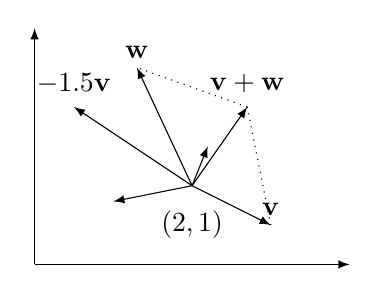
\begin{tikzpicture}
		\draw[-latex] (0,0) -- (0,3);
		\draw[-latex] (0,0) -- (4,0);

		\draw[-latex] (2,1) -- (1,0.8);
		\draw[-latex] (2,1) -- (2.2,1.5);
		%\draw[-latex] (2,1) -- (3,1.25);
		\draw[-latex] (2,1) -- (1.3,2.5); %w
		\draw[-latex] (2,1) -- (3,0.5); %v
		\draw[-latex] (2,1) -- (2.7,2); %v+w
		\draw[-latex] (2,1) -- (0.5,2); %1.5v
		\draw[dotted,thin] (3,0.5) -- (2.7,2);
		\draw[dotted,thin] (2.7,2)-- (1.3,2.5);

		\draw (2,0.5) node{$(2,1)$};
		\draw (3,0.7) node{$\mathbf{v}$};
		\draw (1.3,2.7) node{$\mathbf{w}$};
		\draw (2.7,2.3) node{$\mathbf{v+w}$};
		\draw (0.5,2.3) node{$-1.5\mathbf{v}$};
	\end{tikzpicture}
	\caption{The vector space of all vectors at $(2,1)$, $\mathbb{R}_{(2,1)}^2$}
\end{figure}
\end{frame}

\begin{frame}{Vector Field}
\begin{definition}[Vector Field]
	The vector field $\mathbf{X}$ on $\mathbb{R}^{n+1}$ is a function which assigns to each point of $\mathbb{R}^{n+1}$ a vector at that point.
	That is, $\mathbf{X}(p) = (p,X(p))$.
\end{definition}

For example, $\mathbf{X}(p) = (p,X(p))$ where the associated function of the vector field, $X : \mathbb{R}^2 \to \mathbb{R}^2$ defined by $X(p) = (1,2)$ assigns a constant vector $(1,2)$ at every vector in $\mathbb{R}^2$.

\begin{figure}[h]
	\centering
	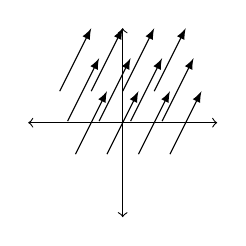
\begin{tikzpicture}[scale=0.4]
		\draw[<->] (-3,0) -- (3,0);
		\draw[<->] (0,-3) -- (0,3);

		\draw[-latex] (1,1) -- (2,3);
		\draw[-latex] (0,1) -- (1,3);
		\draw[-latex] (-1,1) -- (0,3);
		\draw[-latex] (-2,1) -- (-1,3);

		\draw[-latex] (1.25,0.05) -- (2.25,2.05);
		\draw[-latex] (0.25,0.05) -- (1.25,2.05);
		\draw[-latex] (-0.75,0.05) -- (0.25,2.05);
		\draw[-latex] (-1.75,0.05) -- (-0.75,2.05);

		\draw[-latex] (1.5,-1) -- (2.5,1);
		\draw[-latex] (0.5,-1) -- (1.5,1);
		\draw[-latex] (-0.5,-1) -- (0.5,1);
		\draw[-latex] (-1.5,-1) -- (-0.5,1);

	\end{tikzpicture}
	\caption{Vector field with associated function $X(p) = (1,2)$}
\end{figure}
\end{frame}

\begin{frame}{Smooth Vector Field}
\begin{definition}[smooth]
	A function $f : \mathbb{R} \to \mathbb{R}$ is smooth if its partial derivatives of all orders exists and are continuous.
	A function $f : \mathbb{R}^{n+1} \to \mathbb{R}$ is smooth if its component functions $f = (f_1, f_2, \cdots, f_{n+1})$ are smooth.
	A vector field $\mathbf{X}$ is smooth if the associated function $X(p)$ is smooth.
\end{definition}
\end{frame}

\begin{frame}{Gradient of a function}
\begin{definition}[Gradient]
	Let $f : \mathbb{R}^{n+1} \to \mathbb{R}$. Then the gradient of $f$ at $p$ is,
	\begin{equation}
		\nabla f(p) = \left(p,\frac{\partial f}{\partial x_1}(p),\frac{\partial f}{\partial x_2}(p),\cdots,\frac{\partial f}{\partial x_{n+1}}(p)\right)
	\end{equation}
\end{definition}

\begin{block}{$\nabla f(p)$}
	If $f$ is a smooth function, then the gradient of $f$ at $p$ is a smooth vector field.
\end{block}
\end{frame}

\begin{frame}{Example}
	For example, $f : \mathbb{R}^2 \to \mathbb{R}$ defined by $f(x_1,x_2) = 2x_1x_2$ is a smooth function. We have, $\frac{\partial f}{\partial x_1} = 2x_2$ and $\frac{\partial f}{\partial x_2} = 2x_1$. And gradient of $f$ at $(x_1,x_2)$ is $(x_1,x_2,2x_2,2x_1)$. That is, $(2x_2,2x_1)$ at $(x_1,x_2)$.

Calculations : \\
\begin{tabular}{|c|c|c|c|c|c|c|} \hline
	$p$    & $(x_1,x_2)$   & $(0,0)$ & $(1,0)$ & $(0,1)$ & $(-1,0)$ & $(0,-1)$ \\ \hline
	$X(p)$ & $(2x_2,2x_1)$ & $(0,0)$ & $(0,2)$ & $(2,0)$ & $(0,-2)$ & $(-2,0)$ \\ \hline
\end{tabular}

\begin{figure}[h]
	\centering
	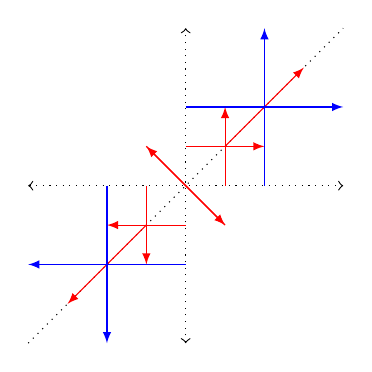
\begin{tikzpicture}[scale=0.5]
		\draw[<->,dotted] (0,-4) -- (0,4);
		\draw[<->,dotted] (-4,0) -- (4,0);
		\draw[dotted] (-4,-4) -- (4,4);

		\draw[-latex,color=red] (1,1) -- (3,3);
		\draw[-latex,color=red] (-1,1) -- (1,-1);
		\draw[-latex,color=red] (1,-1) -- (-1,1);
		\draw[-latex,color=red] (-1,-1) -- (-3,-3);
		\draw[-latex,color=red] (0,1) -- (2,1);
		\draw[-latex,color=red] (0,-1) -- (-2,-1);
		\draw[-latex,color=red] (1,0) -- (1,2);
		\draw[-latex,color=red] (-1,0) -- (-1,-2);

		%\draw[-latex] (-1,2) -- (3,0);
		%\draw[-latex] (2,-1) -- (0,3);
		%\draw[-latex] (1,-2) -- (-3,0);
		%\draw[-latex] (-2,1) -- (0,-3);

		\draw[-latex,color=blue] (0,2) -- (4,2);
		\draw[-latex,color=blue] (2,0) -- (2,4);
		\draw[-latex,color=blue] (-2,0) -- (-2,-4);
		\draw[-latex,color=blue] (0,-2) -- (-4,-2);

		%\draw[-latex] (1,0.5) -- (2,2.5);
		%\draw[-latex] (0.5,1) -- (2.5,2);
		%\draw[-latex] (-1,0.5) -- (0,-1.5);
		%\draw[-latex] (0.5,-1) -- (-1.5,0);
		%\draw[-latex] (1,-0.5) -- (0,1.5);
		%\draw[-latex] (-0.5,1) -- (1.5,0);
		%\draw[-latex] (-1,-0.5) -- (-2,-2.5);
		%\draw[-latex] (-0.5,-1) -- (-2.5,-2);
	\end{tikzpicture}
	\caption{The gradient of $f(x_1,x_2) = 2x_1x_2$}
\end{figure}
\end{frame}

\begin{frame}{Parameterised Curve}
\begin{definition}
	A parameterised curve is a function, $\alpha : I \to \mathbb{R}^{n+1}$ where $I$ is some open interval in $\mathbb{R}$.
	The velocity vector of a parameterised curve $\alpha : I \to \mathbb{R}^{n+1}$ at a point $\alpha(t)$ is the tangent to the curve at that point.
	\begin{equation}
		\dot{\mathbf{\alpha}}(t) = \left(\alpha(t),\frac{d \alpha}{dt} (t)\right)
	\end{equation}
\end{definition}

For example, $\alpha : I \to \mathbb{R}^2$ defined by $\alpha(t) = (2t,t^2)$ is a parameterised curve. We have, $\frac{d\alpha}{dt} = (\frac{dx_1}{dt}(t),\frac{dx_2}{dt}(t)) = (2,2t)$ where $\alpha(t) = (x_1(t),x_2(t))$. The velocity vector at $t = 3$ is $\dot{\alpha}(3) = (\alpha(t),\frac{d\alpha}{dt}) = (6,9,2,6)$.
\end{frame}

\begin{frame}{Integral Curve}
\begin{definition}
	Let $\mathbf{X}$ be a vector field and let $U$ be an open subet of $\mathbb{R}^{n+1}$.
	An integral curve $\alpha$ on $U$ is a parameterised curve, $\alpha : I \to \mathbb{R}^{n+1}$ such that for each $\alpha(t) = p \in U$, the velocity vector $\dot{\alpha}(t)$ is the associated vector $\mathbf{X}(p)$ of the vector field $\mathbf{X}$ at that point. Thus, for each $t \in I$, $\dot{\alpha}(t) = \mathbf{X}(\alpha(t))$.
	\begin{equation}
		\left(\alpha(t),\frac{d \alpha}{dt}(t)\right) = \left(\alpha(t),X(\alpha(t))\right)
	\end{equation}
	Let $X(p) = \left(X_1(p),X_2(p),\cdots,X_{n+1}(p)\right)$ and $\alpha(t) = \left(x_1(t),x_2(t),\cdots,x_{n+1}(t)\right)$. Then, comparing components of the vector at $\alpha(t)$ we get the following system of equations,
	\begin{equation}
		\frac{d x_j}{dt}(t) = X_j(\alpha(t)),\ j = 1,2,\cdots,(n+1)
	\end{equation}
\end{definition}
\end{frame}

\begin{frame}{Example}
For example, Consider $\alpha : (2,3) \to \mathbb{R}^2$ defined by $\alpha(t) = (t,t^2)$. Then $\alpha$ is a parameterised curve in vector field, $\mathbf{X}$ which has the associated function $X(x_1,x_2) = (1,2x_1)$. Then, $\mathbf{X}(x_1,x_2) = (x_1,x_2,1,2x_1)$. And
\[ \dot{\alpha}(t) = \left( \alpha(t),\frac{d\alpha}{dt}(t) \right) = \left( x_1(t),x_2(t),\frac{dx_1}{dt}(t), \frac{dx_2}{dt}(t) \right) = (t,t^2,1,2t) \]
Clearly, $\alpha$ is an integral curve of $\mathbf{X}$ as $\dot{\alpha}(t) = X(\alpha(t))$ for every $t \in (2,3)$.
\end{frame}

\begin{frame}{Integral Curve}
Calculations:\\
\begin{tabular}{|c|c|c|c|c|} \hline
	$p$    & $(0,0)$ & $(1,0)$ & $(0,1)$ & $(1,1)$ \\ \hline 
	$X(p)$ & $(1,0)$ & $(2,2)$ & $(1,1)$ & $(2,3)$ \\ \hline 
	\\ \hline
	$(-1,0)$ & $(0,-1)$ & $(-1,1)$ & $(1,-1)$ & $(-1,-1)$ \\ \hline
	$(0,-2)$ & $(1, 1)$ & $(0,-1)$ & $(2, 1)$ & $( 0,-3)$ \\ \hline
\end{tabular}

\begin{figure}[h]
	\centering
	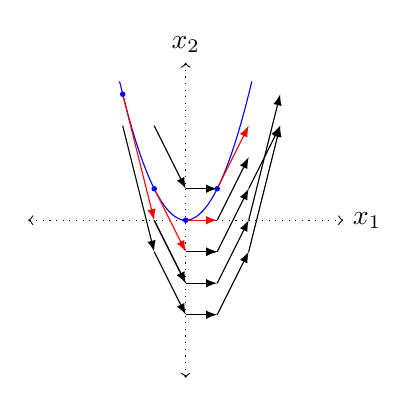
\begin{tikzpicture}[scale=0.4]
		\draw[<->,dotted] (-5, 0) -- (5, 0) node[right] {$x_1$};
  		\draw[<->,dotted] (0,-5) -- (0, 5) node[above] {$x_2$};
  		\draw[domain=-2.1:2.1, smooth, variable=\x, blue] plot ({\x}, {\x*\x});

		\draw[-latex,color=red] (0,0) -- (1,0);

		\draw[-latex] (0,1) -- (1,1);
		\draw[-latex] (1,0) -- (2,2);
		\draw[-latex] (-1,3) -- (0,1);

		\draw[-latex,color=red] (-2,4) -- (-1,0);
		\draw[-latex,color=red] (1,1) -- (2,3);

		\draw[-latex] (0,-1) -- (1,-1);
		\draw[-latex,color=red] (-1,1) -- (0,-1);

		\draw[-latex] (-1,0) -- (0,-2);
		\draw[-latex] (0,-2) -- (1,-2);
		\draw[-latex] (1,-2) -- (2,0);
		\draw[-latex] (2,0) -- (3,4);

		\draw[-latex] (0,-1) -- (1,-1);
		\draw[-latex] (-1,0) -- (0,-2);

		\draw[-latex] (-2,3) -- (-1,-1);
		\draw[-latex] (-1,-1) -- (0,-3);
		\draw[-latex] (0,-3) -- (1,-3);
		\draw[-latex] (1,-3) -- (2,-1);
		\draw[-latex] (2,-1) -- (3,3);

		\draw[-latex] (0,-1) -- (1,-1);
		\draw[-latex] (1,-1) -- (2,1);
		\draw[-latex] (2,1) -- (3,3);

		\node[circle,fill=blue,inner sep=0pt, minimum size=2pt] at (1,1){};
		\node[circle,fill=blue,inner sep=0pt, minimum size=2pt] at (0,0){};
		\node[circle,fill=blue,inner sep=0pt, minimum size=2pt] at (-1,1){};
		\node[circle,fill=blue,inner sep=0pt, minimum size=2pt] at (-2,4){};
\end{tikzpicture}
	\caption{Integral Curve $\alpha(t) = (t,t^2)$ in $\mathbf{X}$ with $X(x_1,x_2) = (1,2x_1)$}
\end{figure}
\end{frame}

\begin{frame}{Unique Integral Curve in Smooth Vector Field}
\begin{theorem}
	Let $\mathbf{X}$ be a smooth vector field on an open set $U \subset \mathbb{R}^{n+1}$ and let $p \in U$.
	Then there exists an open interval $I$ containing $0$ and an integral curve $\alpha : I \to U$ such that
	\begin{enumerate}
		\item $\alpha(0) = p$
		\item If $\beta : \tilde{I} \to U$ is any other integral curve with $\beta(0) = p$, then $\tilde{I} \subset I$ and $\beta(t) = \alpha(t)$, for all $t \in \tilde{I}$.
	\end{enumerate}
\end{theorem}
\end{frame}

\begin{frame}{Proof}
\begin{proof}
	Let $\mathbf{X}$ be a smooth vector field.
	Suppose $\alpha$ be an integral curve in $\mathbf{X}$.
	Then, $\dot{\alpha}(t) = \mathbf{X}(\alpha(t))$.
	Let $x_j(t)$ be the components of $\alpha(t)$ and $X_j(p)$ be the components of $X(p)$.
	\begin{align*}
		\dot{\alpha}(t) & = \left(\alpha(t),\frac{d \alpha}{dt}(t)\right) \\
		& = \left(x_1(t),\cdots,x_{n+1}(t),\frac{dx_1}{dt}(t),\cdots,\frac{dx_{n+1}}{dt}(t)\right)\\
		\mathbf{X}(\alpha(t)) & = (\alpha(t),X(\alpha(t))) \\
		& = \left( x_1(t),\cdots,x_{n+1}(t),X_1(\alpha(t)),\cdots,X_{n+1}(\alpha(t))\right)
	\end{align*}
\end{proof}
\end{frame}

\begin{frame}{Proof}
\begin{proof}
	Thus, we a system of $n+1$ first order differential equations in $n+1$ unknowns satisfying the initial condition $\alpha(0) = p$.
	\begin{align*}
		\frac{dx_1}{dt}(t) & = X_1(\alpha(t)) \\
		\frac{dx_2}{dt}(t) & = X_2(\alpha(t)) \\
		& \vdots \\
		\frac{dx_{n+1}}{dt}(t) & = X_{n+1}(\alpha(t))
	\end{align*}
\end{proof}
\end{frame}

\begin{frame}{Proof}
\begin{proof}
	By the theorem on solution of systems of first order ordinary differential equations, there exists an interval $I$ containing $0$ and a solution --- a family of functions $\{ x_1(t), x_2(t), \cdots,x_{n+1}(t)\}$ satisfying the above system of equations satisfying the initial condition $\alpha(0) = p$.

	Define $\alpha : I \to U$ using the component functions of $\alpha$ as $x_j$s in the above solution. Then, we have a integral curve of the vector field $\mathbf{X}$ satifying the initial condition $\alpha(0) = p$.

	Let $\beta : \tilde{I} \to U$ be another integral curve with $\beta(0) = p$. Then by the uniqueness of the solution for the system of first order ordinary differential equations with an initial condition, $\beta(t) = \alpha(t)$ for every $ t \in I \cup \tilde{I}$.
\end{proof}
\end{frame}

\begin{frame}{Proof}
	\begin{proof}
	Let $\{\beta_1,\beta_2,\cdots\}$ be the family of integral curves with $\beta_j : I_j \to U$ satisfying $\beta_j(0) = p$. Consider $I = \bigcup\limits_{j \in \mathbb{N}} I_j$.

	Define $\alpha : I \to U$ by $\alpha(t) = \beta_j(t)$ where $t \in I_j$ for some $j \in \mathbb{N}$. Then $\alpha$ is well-defined and is a maximal integral curve in $\mathbf{X}$ such that $\alpha(0) = p$.
\end{proof}
\end{frame}

\begin{frame}{Complete Vector Field}
\begin{definition}
	A smooth vector field $\mathbf{X}$ on $U \subset \mathbb{R}^{n+1}$ is \textbf{complete} if for every $p \in U$, the maximal integral curve through $p$ has domain equal to $\mathbb{R}$.
\end{definition}
\end{frame}

\begin{frame}{Divergence of a Vector Field}
\begin{definition}
	The \textbf{divergence} of a smooth vector field $\mathbf{X}$ on $U \subset \mathbb{R}^{n+1}$ is the function $div\ \mathbf{X} : U \to \mathbb{R}$ defined by
	\[ div\ X(x_1,x_2,\cdots,x_{n+1}) = \sum_{i=1}^{n+1} \frac{\partial X_i}{\partial x_i} \]
	where $X_i$ are the component function of the associated function $X$ of the vector field $\mathbf{X}$.
\end{definition}

For example, Consider $\mathbf{X}$ with associated function $X : \mathbb{R}^2 \to \mathbb{R}^2$ defined by $X(x_1,x_2) = (2x_1,x_1x_2)$. Then $div\ \mathbf{X}(x_1,x_2) = \frac{\partial X_1}{\partial x_1} + \frac{\partial X_2}{\partial x_2} = 2 + x_1$.
\end{frame}

\begin{frame}{Local 1-parameter Group}
	\begin{definition}[Local 1-parameter Group]
		Let $\mathbf{X}$ be a smooth vector field on $U$, $U \subset \mathbb{R}^{n+1}$. Let $\phi_t(p) = \alpha_p(t)$ where $\alpha_t$ is the maximal integral curve of $\mathbf{X}$ through $p$. Then $\phi_t$ together with function composition is a group. And is called the local $1$-parameter group associated with $\mathbf{X}$.
	\end{definition}
\end{frame}

\end{document}
